\documentclass[12pt,a4paper]{article}

\usepackage{geometry}
\geometry{a4paper,left=20mm,top=20mm}

\usepackage{amssymb}
\usepackage{graphicx}
\usepackage{ulem}
%\usepackage{algorithmic,amssymb,graphicx,amssymb,amsmath,psfig,epsfig,multirow,url,arcs,proof}
\usepackage{subfigure}
\usepackage{float}

\usepackage[usenames, dvipsnames]{color}
% \usepackage[nodots]{numcompress}
\usepackage[linesnumbered,ruled]{algorithm2e}
\usepackage{lineno}
\usepackage{hyperref}


\SetKwProg{Fn}{Function}{}{\\}
\SetKwComment{Comment}{start}{end}
\SetKw{Continue}{continue}

\newtheorem{defn}{Definition}
\newtheorem{theorem}{THEOREM}[section]
\newtheorem{lemma}[theorem]{LEMMA}
\newtheorem{proposition}[theorem]{PROPOSITION}
\newtheorem{obs}[theorem]{OBSERVATION}
\newtheorem{corollary}[theorem]{COROLLARY}
\newtheorem{conjecture}[theorem]{CONJECTURE}

\newenvironment{example}[1][Example]{\begin{trivlist}
\item[\hskip \labelsep {\bfseries #1}]}{\end{trivlist}}
\newenvironment{remark}[1][Remark]{\begin{trivlist}
\item[\hskip \labelsep {\bfseries #1}]}{\end{trivlist}}

\setlength\linenumbersep{3pt}

% \journal{Computer \& Graphics}

\title{Surface Reconstruction}
\author{Ashok Dhungana, Prabhav Adhikari, Suraj Yadav}
%\address{National Institute of Technology Calicut}
\begin{document}
%\begin{frontmatter}

%% Title, authors and addresses

%% use the tnoteref command within \title for footnotes;
%% use the tnotetext command for the associated footnote;
%% use the fnref command within \author or \address for footnotes;
%% use the fntext command for the associated footnote;
%% use the corref command within \author for corresponding author footnotes;
%% use the cortext command for the associated footnote;
%% use the ead command for the email address,
%% and the form \ead[url] for the home page:
%%
%% \title{Title\tnoteref{label1}}
%% \tnotetext[label1]{}
%% \author{Name\corref{cor1}\fnref{label2}}
%% \ead{email address}
%% \ead[url]{home page}
%% \fntext[label2]{}
%% \cortext[cor1]{}
%% \address{Address\fnref{label3}}
%% \fntext[label3]{}

%% use optional labels to link authors explicitly to addresses:
%% \author[label1,label2]{<author name>}
%% \address[label1]{<address>}
%% \address[label2]{<address>}

%\begin{titlepage}
%	\begin{center}
%		\textup{\small {\bf CS4089 Project} \\ \bf Report}\\[0.2in]
%		
%		% Title
%		\Large \textbf {Surface Reconstruction}\\[0.5in]
%		
%		\small \emph{Submitted in partial fulfillment of\\
%			the requirements for the award of the degree of}
%		\vspace{.2in}
%		
%		{\bf Bachelor of Technology \\in\\ Computer Science and Engineering}\\[0.5in]
%		
%		% Submitted by
%		\normalsize Submitted by \\
%		\begin{table}[h]
%			\centering
%			\begin{tabular}{lr}\hline \\
%				Roll No & Names of Students \\ \\ \hline
%				\\
%				B130055CS & Ashok Dhungana \\
%				B130056CS & Prabhav Adhikari \\ 
%				B130487CS & Suraj Yadav \\ \\ \hline 
%			\end{tabular}
%		\end{table}
%		
%		\vspace{.1in}
%		Under the guidance of\\
%		{\textbf{Subhasree M}}\\[0.2in]
%		
%		\vfill
%		
%		% Bottom of the page
%		
\includegraphics[width=0.18\textwidth]{images/nitc-logo}\\[0.1in]
%		\Large{Department of Computer Science and Engineering}\\
%		\normalsize
%		\textsc{National Institute of Technology Calicut}\\
%		Calicut, Kerala, India -- 673 601 \\
%		\vspace{0.2cm}
%		Winter Semester 2017
%		
%	\end{center}
%	
%\end{titlepage}
%
%\newpage
%\thispagestyle{empty}
%
%\begin{center}
%	
%	\huge{Department of Computer Science and Engineering}\\[0.5cm]
%	\normalsize
%	\textsc{National Institute of Technology Calicut}\\[2.0cm]
%	
%	\emph{\LARGE Certificate}\\[2.5cm]
%\end{center}
%\normalsize This is to certify that this is a bonafide record of the project presented by the students whose names are given below in partial fulfilment of the requirements of the degree of Bachelor of Technology in Computer Science and Engineering.\\[1.0cm]
%
%\begin{table}[h]
%	\centering
%	\begin{tabular}{lr}
%		Roll No & Names of Students \\ \\ \hline
%		\\
%		B130055CS & Ashok Dhungana \\ 
%		B130056CS & Prabhav Adhikari \\
%		B130487CS & Suraj Yadav \\
%	\end{tabular}
%\end{table}
%
%\vfill
%
%
%% Bottom of the page
%\begin{flushright}
%	Subhasree M\\
%	(Project Guide)\\[1.5cm]
%	Anu Mary Chacko\\
%	(Course Coordinator)\\
%\end{flushright}
%
%\begin{flushleft}
%	Date: \date{}
%\end{flushleft}

\newpage
\vspace{2in}
\begin{abstract}
Given a finite sampling $S$ of an unknown surface $F$, Surface Reconstruction is concerned with the calculation of a model of $F$ from $S$. In this report we present our algorithm that generates a manifold triangular mesh $F$ from a set of unorganized points and compare it with various existing algorithms for Surface Reconstruction. 
\end{abstract}

%\begin{keyword}
%Surface reconstruction \sep Delaunay Triangulation \sep Voronoi Diagram \sep Point sets
%%% MSC codes here, in the form: \MSC code \sep code
%%% or \MSC[2008] code \sep code (2000 is the default)
%
%\end{keyword}
%
%\end{frontmatter}

%%
%% Start line numbering here if you want
%%

\newpage
\tableofcontents

\newpage
\listoffigures

\section{Preliminaries}

\subsection{Convex Hull} Given a set of points $P$, a closed convex polygon that includes all the points in $P$ with the least area.

\subsection{Triangulation}
Triangulation of a set of points $P$ is the subdivision of the convex hull of the points into simplices such that any two simplices intersect in a common face of any dimension or not at all and such that the set of vertices of the simplices are contained in $P$. Every point set has a triangulation. 

\subsection{Delaunay Triangulation}
Delaunay triangulation of $P$ is a triangulation of $P$ in which every triangle is Delaunay. A triangle is delaunay if its vertices are in $P$ and its open circumdisk is empty. For a given point set, there always exists a delaunay triangulation, and is unique if and only if no four points in $P$ lie on a common empty circle.

\subsection{Voronoi Diagram}
The partitioning of a plane with point set $P$, into convex polygons such that each polygon contains exactly one generating point in $P$ and every point in a given polygon is closer to its generating point than to any other. Voronoi Diagram is dual to the Delaunay triagulation of the point set.

%\subsection{Combinatorial Map}
%A (2-dimensional) oriented combinatorial map, or just map, $M$, is a triple $D$, $\theta_0$ , $\theta_1$ , where $D$ is a finite set of elements, called darts, $\theta_0$ is an involutory bijection on $D$, and $\theta_1$ is a bijection on $D$. We may also assume that $\theta_0$ has no fixed points.
%
%\subsection{Gabriel graph}
%Gabriel graph is the graph with vertex set $S$ in which any points $P$ and $Q$ in $S$ are adjacent precisely if they are distinct and the closed disc (or sphere in $3D$) of which line segment $PQ$ is a diameter contains no other elements of $S$.

\subsection{Euclidean minimum spanning tree}
The Euclidean minimum spanning tree or EMST is a minimum spanning tree of a set of n points in the plane (or more generally in ℝd), where the weight of the edge between each pair of points is the Euclidean distance between those two points.

\subsection{Medial Axis}
The Medial Axis (MA) of subset $S$ bounded by curve $C$, is defined as the locus of the centers of circles (in $\mathbb{R}^2$), spheres (in $\mathbb{R}^3$), that are tangent to curve $C$ in two or more points, where all such circles (or spheres) are contained in $S$.

The medial axis together with the associated radius of the inscribed discs is called the Medial Axis Transform (MAT).


\begin{figure}[!h]
	\centering
	\subfigure[\label{fig:boundarySample}]{
		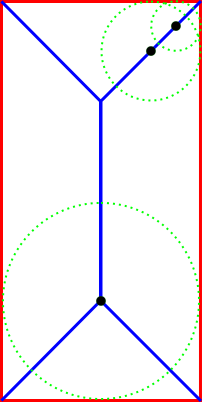
\includegraphics[height=1.8in,width=0.9in]{images/MAT1}
	}
%	\subfigure[\label{fig:DotPattern}]{
%		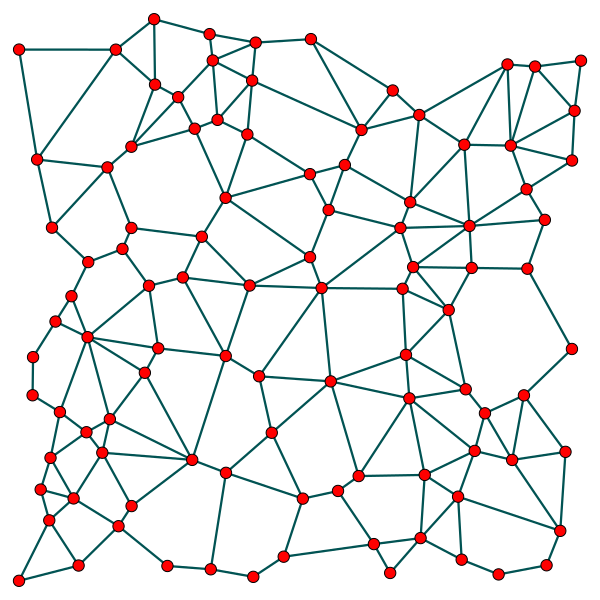
\includegraphics[height=1.8in,width=1.8in]{images/Gabriel_graph}
%	}
	\caption{
		(a) MAT (\textcolor{red}{\protect\uline{Original Shape}}, \textcolor{green}{\protect\dotuline{Tangent Circles}}, \textcolor{blue}{\protect\dashuline{MAT}}). 
%		(b) Gabriel Graph of Random Points.
	}
\end{figure}

\normalem
\section{Literature Survey}

An early, and influential, attempt to characterize the shape of a set of points is due to \cite{Edelsbrunner:2006:SSP:2263365.2270180}, which introduced a construction known as "$\alpha-shape$" as a generalization of the convex hull. For a finite set $P$ of points in the plane, the "$\alpha-hull$" for "$\alpha = 0$" is the intersection of all closed discs of radius $1/\alpha$ containing all the points of $P$ (where for negative values of $\alpha$ a closed disk of radius, $1/\alpha$ is interpreted as the complement of an open disk of radius $1/\alpha$). As $\alpha$ approaches 0, the $\alpha-hull$ approaches the ordinary convex hull, and therefore the $0-hull$ is stipulated to be the convex hull. The $\alpha-shape$ is a straight-line graph (usually a polygon) derived in a straightforward manner from the $\alpha-hull$. When $\alpha = 0$, this is the convex hull, and for large negative values of $\alpha$ it is $P$ itself.


A related notion, $A-shape$, was introduced in \cite{Melkemi:7693802}. Given a finite set of points P, and a set A (which evidently needs to be disjoint from P, although the authors do not specify this), we can define the $A-shape$ of $P$ by first constructing the Voronoi diagram for $A \cup P$ and then joining together any pair of points $p, q \in P$ whose Voronoi cells both border each other and border some common Voronoi cell containing a point of $A$. The edges $p-q$ belong to the Delaunay triangulation of $A \cup P$ : they are the "$A-exposed$" edges of the triangulation. An important
issue discussed in the paper is how to choose $A$ so that the $A-shape$ of $P$ is "adequate." In a later paper \cite{fadili:hal-01123869}, the $A-shape$ is used as the basis for an "onion-peeling" method, by analogy with the popular convex onion-peeling method for organizing a set of points and extracting a "central" embedded convex shape from them \cite{Chazelle1057060}.


Two rather different constructs, $r-shape$ and $s-shape$, were defined in \cite{Chaudhuri:1997:NAC:269777.269779} as follows. The initial set of points $P$ is assumed to be a dot pattern, that is, a planar point set whose elements are “clearly visible as well as fairly densely and more or less evenly distributed.” To obtain the $s-shape$, the plane is partitioned into a lattice of square cells of side-length $s$. The $s-shape$ is simply the union of lattice cells containing points of $P$. The authors suggest a procedure for optimizing the value of $s$ so that the $s-shape$ best approximates the perceived shape of the dot pattern. For the $r-shape$, they first construct the union of all disks of radius $r$ centered on points of $P$. For points $p, q \in P$ , the edge $p-q$ is selected if and only if the boundaries of the disks centered on $p$ and $q$ intersect in a point which lies on the boundary of the union of all the disks. The $r-shape$ of $P$ is the union of the selected edges, and the authors show that this can be computed in time $O(n)$, where $n$ is the cardinality of $P$. They note that the $r-shape$ is a subgraph of the $\alpha-shape$ in the sense of \cite{Edelsbrunner:2006:SSP:2263365.2270180}. Regarding the selection of $r$, they note that "to get a perceptually acceptable shape, a suitable value of $r$ should be chosen, and there is no closed form solution to this problem," and that moreover "‘perceptual structure’ of $P$ ... will vary from one person to another to a small extent."

The use of Voronoi diagrams for constructing regions from point-sets has also been advocated in the context of GIS \cite{Harith01}. In this context, the set $P$ consists of points known to be in a certain region, for which an approximation to the boundary is required. It is assumed that in addition to $P$ another point-set $P'$ is given, consisting of points known to lie outside the region to be approximated. From the Voronoi diagram for $P \cup P'$, the method simply selects the union of the Voronoi cells containing points of $P$. The resulting shape differs from the characteristic shapes constructed in this paper in that the original point-set lies entirely in its interior. Depending on one’s purposes,
this feature may either be desirable or undesirable. 


A similar method \cite{Avi-04} is based on Delaunay triangulations. Given sets $P$ and $P'$ as before, the Delaunay triangulation of $P \cup P'$ is constructed, and then the midpoint of every edge which joins a point in $P$ to a point in $P'$ is selected. The final region is produced by joining all pairs of selected midpoints belonging to edges of the same triangle.

%\section{Detailed Study of Some papers} 
%\subsection{Recursive Voids for Identifying a Nonconvex Boundary
%of a Set of Points in the Plane \cite{recVoid}}
%
%A method that identifies the boundary of a nonconvex shape of a set of points,$P$ in the plane is introduced in this paper. The boundary of the shape is explored through finding empty regions recursively within a shell that encapsulates all of the points. This algorithm is output sensitive and runs in linear $O(ln)$ time determined by the output parameter $l$, which is proportional to the length of the nonconvex boundary measured by a threshold unit distance. The recursive nature of the algorithm allows a tree structure that characterizes the empty regions, and by complementarity, the nonconvex shape itself. 
%
%This work falls under the non-Delaunay methods.The algorithm focuses on identifying the empty regions within a shell $H$ that encapsulates $P$, such as the convex hull of $P$. In exploring these empty regions, a unique boundary is defined
%between the points in $P$ and a given empty region, with respect to an edge E,
%such that this boundary together with edge E define an empty simple polygon, which is called a void. Then, recursively new voids are created by exploring edges on the boundary that are greater than or equal to some threshold $t$.
%
%\subsection{Efficient generation of simple polygons for characterizing the shape of a set of points in the plane \cite{Duckham:2008:EGS:1385702.1385955}}
%
%For a finite set of at least three points in the Cartesian plane $P \subset \mathbb{R}^2$ , the characteristic shape algorithm yields a possibly non-convex area with a shape that characterizes the distribution of the input point set. All the sets under consideration in this paper are sets of points in the Cartesian plane ${R}^2$, and these sets are assumed to be finite. 
%
%
%The $\chi$-shape produced by the algorithm has the properties that:
%\begin{enumerate}
%	\item it is a simple polygon;
%	\item it contains all the points of $P$ ; and
% 	\item it bounds an area contained within and possibly equal to the convex hull of the points of $P$.
%\end{enumerate}
%
%\begin{figure}[!h]
%	\centering
% 	\subfigure[\label{fig:chiShape1}]{
%		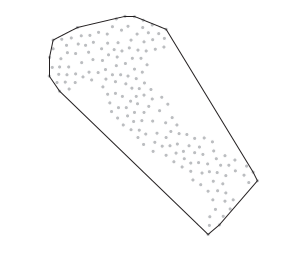
\includegraphics[height=1.5in,width=1.0in]{images/chi1}
% 	}
% 	\subfigure[\label{fig:chiShape2}]{
%		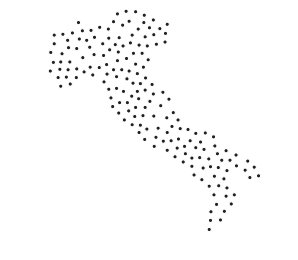
\includegraphics[height=1.5in,width=1.0in]{images/chi2}
% 	}
% 	\subfigure[\label{fig:chiShape3}]{
%		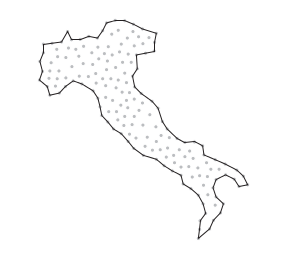
\includegraphics[height=1.5in,width=1.0in]{images/chi3}
% 	}
%	\caption{
%		(a) Convex Hull of $P$. (b) Point Set $P$. (c) Characteristic $\chi$ shape of $P$.
%	}
%\end{figure}
%
%
%\begin{itemize}
%	\item \textbf{Idea} The $\chi$-shape algorithm is based on "shaving" exterior edges (edges that bound only one triangle) from a triangulation of the input point set in order of the length of edges and subject to a regularity constraint. The algorithm itself has a time complexity of $O(n\log n)$, where $n$ is the number of input points.
%
%	\item \textbf{Algorithm}
%The algorithm can be summarized as comprising the following steps for an input point set $P$ and a length parameter $l$:
%\begin{enumerate}
%	\item Generate the \textbf{Delaunay triangulation}, $\tau$ of the set of input points $P$;
%    \item Construct a priority list of boundary edges $B$. The checking for boundary edge can be done using idea from \textbf{Combinatorial Map}.
%	\item Remove the longest boundary edge from the triangulation, $\tau$ such that:
%	\begin{enumerate}
%		\item the edge to be removed is longer than the length parameter $l$; and
%		\item the exterior edges of the resulting triangulation form the boundary of a simple polygon and the triangulation, $\tau$ is regular;
%    \end{enumerate}
%    \item Repeat 2. as long as there are more edges to be removed
%	\item Return the polygon formed by the exterior edges of the triangulation
%\end{enumerate}
%\end{itemize}
%
%\subsection{Power Crust}
%\textbf{Power Crust} \cite{Amenta:2001:PC:376957.376986} is a construction which takes a sample of points from the surface of a three-dimensional object and produces a surface mesh and an approximate medial axis.
%\begin{itemize}
%	\item \textbf{Idea} The approach is to first approximate the medial axis transform (MAT) of the object, then use an inverse transform to produce the surface representation from the MAT.
%	\item \textbf{Algorithm} 
%		\\
%		Let $F$ be the original surface and $S$ the sampled points from the surface.
%        \begin{enumerate}
%        \item Compute the Voronoi diagram of the sample points $S$.
%		\item For each sample point $s$, compute its poles. Poles of a sample point $s\in S$ are the farthest vertex of its Voronoi cell in the interior and the of exterior of $F$. 
%        \item Compute the power diagram (a weighted Voronoi diagram using input parameter $\rho$) of the poles.
%        \item Label each pole either inside or outside $F$.
%        \item Output the power diagram faces separating the cells of inside and outside poles as the \textbf{Power Crust}.
%        \item Output the regular triangulation faces connecting inside poles as the \textbf{Power Shape}.
%        \end{enumerate}
%		The \textbf{Power Shape} approximates the \textbf{MAT} of $F$, while \textbf{Power Crust} approximates the $F$.
%\begin{figure}[!h]
%	\centering
%	\subfigure[\label{fig:crust1}]{
%		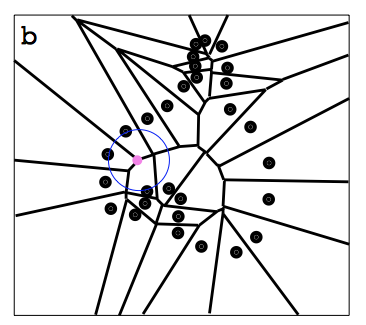
\includegraphics[height=0.7in]{images/crust1}
%	}
%	\subfigure[\label{fig:crust2}]{
%		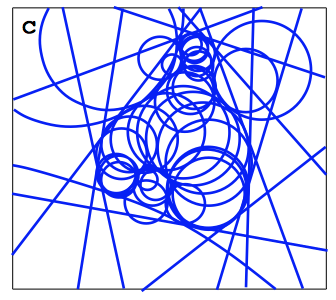
\includegraphics[height=0.7in]{images/crust2}
%	}\\
%	\subfigure[\label{fig:crust3}]{
%		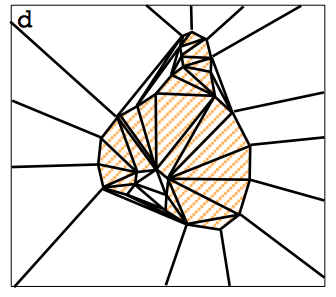
\includegraphics[height=0.7in]{images/crust3}
%	}
%	\subfigure[\label{fig:crust4}]{
%		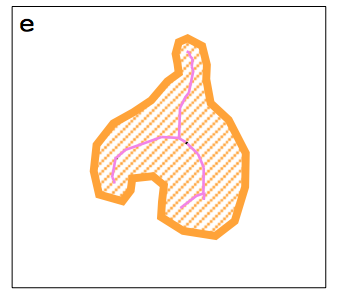
\includegraphics[height=0.7in]{images/crust4}
%	}
%	\caption{
%		(a) The Voronoi diagram of S, with the net ball surrounding one pole shown. (b) The inner and outer polar balls. (c) The power diagram cells of the poles. (d) The power crust and the power shape.
%	}
%\end{figure}
%\end{itemize}
%
%\subsection{Shape-Hull}
%\textbf{Shape-Hull}\cite{Peethambaran:2015:RWS:2941001.2941130} is a non-parametric, single stage Delaunay sculpting algorithm which reconstructs topologically correct piece-wise linear approximation for divergent concave surfaces.
%
%\begin{itemize}
%	\item \textbf{Idea} For a given set of Points $S \in \mathbb{R}^2$ S is sampled	from a divergent concave curve $\sum_D$, a proximity graph called as shape-hull graph $SHG(S)$ is defined that contains all Gabriel edges and a few non-Gabriel edges of the Delaunay triangulation of $S$. Shape-hull $SH(S)$ is defined as the boundary of Shape-hull graph $SHG(S)$. Under dense sampling assumption it can be shown that $SH(S)$ represents a piece-wise linear approximation of $\sum_D$.
%	
%	\item \textbf{Algorithm}\\
%    We define a tetrahedral $T$ to be \textbf{deletable} if either 
%    \begin{enumerate}    
%    \item It has only one face $f$ on the boundary and the vertex opposite $f$ is not on the boundary
%    \item It has exactly two face $f_1 and f_2$ on the boundary and the edge opposite to common edge of $f_1 and f_2$ is not on the boundary. 
%    \end{enumerate}
%     Let $S$ be the sampled points set.
%     \begin{enumerate}
%     \item Set $D$ =  $Del(S)$ (Delaunay Triangulation of $S$).
%     \item Set $PQ$ = Priority Queue,  containing \textbf{deletable} boundary tetrahedral of $D$, sorted in the descending order of their circumradii.
%     \item While PQ is not empty
%     	\begin{enumerate}
%        	\item $T$  = $pop(PQ)$. 
%            \item If $T$ is \textbf{deletable} and circumcenter of $T$ lies outside the boundary of $D$ \textbf{then}
%			\begin{itemize}
%				\item delete $T$ from $D$
%				\item add the \textbf{deletable} neighbors of $T$ to $PQ$.
%			\end{itemize}
%        \end{enumerate}
%	\item Finally $D$ is  reconstructed surface.
%    \end{enumerate}
%    
%    \item \textbf{Complexity}\\
%    In $\mathbb{R}^3$, Delaunay triangulation takes $\mathcal{O}(n^2\log{}n)$ in the worst case\cite{Boissonnat:1984:GST:357346.357349}. Let $t_c$ = number of Delaunay tetrahedral in the Convex hull of $S$ and $t_d$ = number of tetrahedral in the reconstructed surface. Each push/pop operation take $\mathcal{O}(\log{}n)$ time, while the boundary  checking and deletion of tetrahedral can be done in constant time. Thus for a given $Del(S)$, it takes $k\mathcal{O}(\log{}n)$ time to reconstruct the surface. For surfaces having large concave portion, k tends to be large and as a result, the reconstruction time will be substantially increased. However, the worst case time complexity of shape-hull algorithm is $\mathcal{O}(n^2\log{}n)$, dominated by $Del(S)$ construction.
%\end{itemize}
%\begin{figure}[!h]
%	\centering
%	\subfigure[\label{fig:shapehull1}]{
%		
\includegraphics[height=1.5in]{images/shapehull1}
%	}
%	\subfigure[\label{fig:shapehull2}]{
%		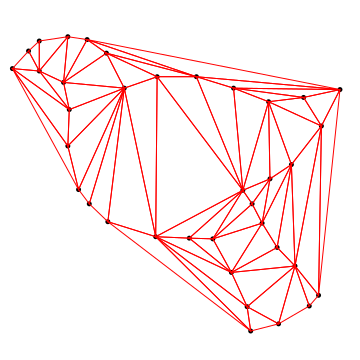
\includegraphics[height=1.5in]{images/shapehull2}
%	}
%	\subfigure[\label{fig:shapehull3}]{
%		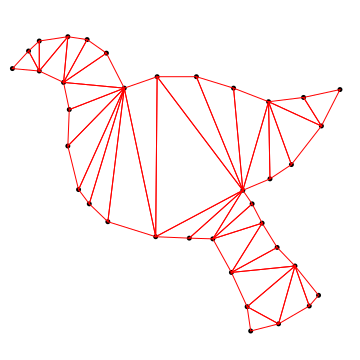
\includegraphics[height=1.5in]{images/shapehull3}
%	}
%	\subfigure[\label{fig:shapehull4}]{
%		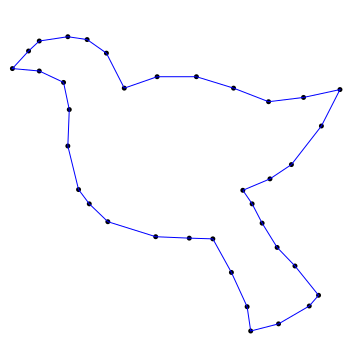
\includegraphics[height=1.5in]{images/shapehull4}
%	}
%	\caption{
%		(a) Sample Points. (b) Delaunay Triangulation. (c) Shape-hull graph. (d) Shape-hull.
%	}
%\end{figure}

\section{Algorithm}

We start with Delaunay tetrahedralization $DT$ of available points in $\mathbb{R}^3$. We use the 3D Delaunay to obtain Euclidean Minimum Spanning Tree of $DT$ using Kruskal's  algorithm.

\subsection{Definitions}

\subsubsection{Hole Graph}Graph induced by the edges of the surface whose edge degree is 1 and of EMST whose edge degree is less than or equal to 1.

\subsubsection{Hole}A connected component in hole graph. A hole is a cycle. 

\subsubsection{Stitching Edges} A subset of edges of all the possible edges in a hole which satisfies the following conditions:
\begin{itemize}
	\item Length of the edge is less than 2 times the minimum of the maximum length edge incident on the vertices of given edge
	\item The edge does not overlap with the existing edges and adjacent faces  
\end{itemize}

\subsubsection{Score} Score of a face is defined as the minimum angle of the face.

\subsubsection{Possible Faces} Given an edge (u,v) the possible faces are each (u,v,w) for w $ \in $ (Adjacent vertices of $ u $ in $ Surface  $ $ \cup $ Adjacent vertices of $ v $ in $Surface $)

\subsubsection{PQ} PQ is a priority queue with key as score of a face and value as the edge and point pair representing the face. The priority queue is sorted in descending order.

\subsubsection{Face Acceptance Condition} A face satisfying following conditions are accepted into the surface:
\begin{itemize}
	\item Either all the edges of the face must have edge degrees less than 2 or each edge with edge degree 2 must be able to replace a face adjacent to it
	\item Number of edges in the face with edge length less than max length of EMST edge should be greater than or equal to edge condition integer
\end{itemize}

\begin{algorithm}
	\caption{Surface Reconstruction using Euclidean MST }

	\Fn{reconstruct(P) \tcp*[f]{$ P $: Point Set}}{
		$ DT \leftarrow$ Delaunay triangulation of $ P $\\
		$ G \leftarrow $ graph of MST of $ DT $\\
		$ S \leftarrow $ surface initialized with $ \phi  $\\
		$ PQ \leftarrow maxHeap(score,{edge,point}) $ \\
		\tcp{$ score $ is the minimum angle of a $ \triangle $}
		$ edgeCondition \leftarrow 2 $ \\
		\Repeat{$ G` = G $}{
			$ G` \leftarrow G $ \\
			$ stitchEdges \leftarrow getFacesFromEdges(G, DT) $ \\
			$ PQ \leftarrow PQ \cup getFacesFromEdges(G, sticthEdges)$ \\
			$ PQ \leftarrow addToSurface(S, G, PQ, edgeCondition) $ \\
			$ edgeCondition \leftarrow edgeCondition -1$ \\
		}
		$ PostProcess(S,G) $
	}
	
	\Fn{isEdgeOverlap(e,G)}{
		\Return $ true $ if $ e $ has projection on any of the faces adjacent to vertices of $ e $ in $ G $\\
		\Return $ false $ otherwise\\		
	}

	\Fn{getFacesFromEdges(G, edgeSet)}{
		$ faces \leftarrow \phi $ \\
		\ForEach{$ e(u,v) \in edgeSet $}{
			$ pointSet \leftarrow N_{G}[u] \cup N_{G}[u] \setminus \{u,v\} $ \\
			\ForEach{$ w \in pointSet $}{
				$ faces \leftarrow faces \cup \{score of \{u,v,w\}, e, w\} $ \\
			}
		}
		return $ faces $
	}

	\Fn{getStitchEdges(G, DT)}{
		$ H \leftarrow G[\{u,v \mid faceDegree(u,v)\le 1\}]$ \\
		$ sticthEdges\leftarrow \phi $ \\
		\ForEach{$ e(u,v) \in DT \setminus H$ (sorted by length)}{
		\If{$ u,v \in $ same component in $ H $ $ \wedge $ $ e.length \le 2 \times \min(maxLength(u), maxLength(v)) $ $ \wedge $ $\neg edgeOverlap(e)$ $ \wedge $
		($\neg u.covered$ $\vee$ $\neg v.covered $) }{
			$ sticthEdges\leftarrow sticthEdges \cup \{e\}) $\\
			$ u.covered \leftarrow  True $\\ 
			$ v.covered \leftarrow  True $\\}
		}
		\Return sticthEdges
	}
\end{algorithm}

\begin{algorithm}
	\setcounter{AlgoLine}{44}
	\Fn{addToSurface(S,G,PQ,edgeCondition)}{
		$ tempPQ \leftarrow \phi $\\
		\While{$ PQ \ne \phi $}{
			$ score, edge_{0}, point_{0} \leftarrow PQ.pop() $\\
			$ face \leftarrow \{ edge, point\} $ \\
			\If{$ face \in S $}{\Continue}
			$ edge_{1},edge_{2} \leftarrow face \setminus \{edge_{0}\} $ \\
			$ point_{1}, point_{2} \leftarrow $ opposite points of $ edge_{1} $ and $ edge_{2} $ in $ face $ \\
			Check if it is possible to add face to $ edge_{i}'s $ FaceAdjList such that either $ faceEdgeDegree \le 1 $ or if $ face $ can remove any face $ f_{b} $ in FaceAdjList such that $ f_{a} $ is the other face in $ FaceAdjList $ and $ angle(face, f_{a}) < angle(f_{a},f_{b}) $ \\
			\If{false}{continue}
			$ removedFaces \leftarrow $ faces removed \\
			\If{$ \exists f` \in (N_{G}[face] \setminus removedFaces) \mid f`$ overlaps with $face$ }{\Continue}
			\If{count(edges of $ face $ with length $ <= $ max Edge Length in $ MST $) $ \le edgeCondition $}{
				$ tempPQ \leftarrow tempPQ \cup \{score, edge_{0}, point_{0}\} $ \\
				\Continue
			}
			$ S\leftarrow S \cup face $ \\		
			$ G\leftarrow G \cup {face} $ \\
			$ PQ \leftarrow PQ \cup getFacesFromEdges(G, face)$
		}
		\Return $ tempPQ $
	}

	\Fn{PostProcess(G, S)}{
		$ H \leftarrow G[\{u,v \mid faceDegree(u,v)\le 1\}]$ \\
		\ForEach{$ cycle \in H $}{
			\Repeat{$ |cycle| \le 3 $}{
				$ edge_{0}, edge_{1} \leftarrow $ pair of adjacent Edges in $ cycle $ with min angle \\
				$ S \leftarrow S \cup face(edge_{0}, edge_{1}) $ \\
				$ G \leftarrow G \cup \{edge_{0}, edge_{1}\} $ \\
				$ cycle \leftarrow cycle \setminus \{edge_{0} \cap edge_{1}\}$
			}
			$ S \leftarrow S \cup cycle $ \\
			$ G\leftarrow G \cup cycle $ \\
		}
	}
\end{algorithm}


%\begin{algorithm}
%	\caption{Surface Reconstruction using EMST}
%	Get $ Hole Graph $\\
%	Put $ Stitching Edges $ for each hole\\
%	Add all $ possible faces $ with $ score $ in $ PQ $\\
%	\While{$ PQ \ne \phi $}{
%		\If{$ face $ satisfies $ face-conditions $}{add possible neighbouring faces to PQ}
%		\If{$ face $ rejected due to edge condition}{add it to $ PQ' $}
%		$ Surface = Surface \cup face $
%	}
%	$ PQ =  PQ' $	\\
%	Repeat till no change in $ Surface $\\
%	Post-process remaining $ holes $\\
%	
%\end{algorithm}
%
%\begin{algorithm}
%$pts$ $\leftarrow$ get Input Points\\
%$dt$ $\leftarrow$ Delaunay triangulation of $pts$\\
%$possibleEdges$ $\leftarrow$ edges from $dt$\\
%$possibleFaces$ $\leftarrow$ faces from $dt$\\
%$initEdges$ $\leftarrow$ get Euclidean MST from $ dt $\\
%$pq$ $\leftarrow$ $ priorityQueue(score,\{edge,point\}) $\\
%\While{$ surface $ is changed}{
%	$ holeGraph \leftarrow dt $[edges with degree 1]\\
%	$ nextEdges \leftarrow \phi $\\
%	\ForEach { $ e(u,v) \in possibleEdges $}{
%		\If{$ u,v \in $ same component in $ holeGraph $ $ \wedge $ $\neg edgeOverlap(e)$ $ \wedge $
%		 ($\neg u.covered$ $\vee$ $\neg v.covered $) $ \wedge $ $ e.length \le 2 \times \min(maxLength(u), maxLength(v)) $}{
%		 $ nextEdge.insert(e) $\\
%		 $ u.covered \leftarrow  True $\\ 
%		 $ v.covered \leftarrow  True $\\}	
%	}
%	\ForEach{$ e \in initEdges \cup nextEdges $}{
%		\ForEach{$ f \in getFacesFromEdge(e) $}{
%			$ pq.insert(f.score,\{e,f \setminus e\}) $	
%		}	
%	}
%	$ tempPQ \leftarrow \phi $\\
%	\While{$ pq \ne \phi $}{
%		$ score, edge, point \leftarrow pq.pop() $\\
%		$ face \leftarrow \{edge,point\} $\\
%		\If{$ face \in surface $}{continue}
%		$ mustDiscard \leftarrow ValidToAdd(face) $\\
%		\If{$ face \in mustDiscard $}{continue}
%		\If{$ count(edges \in face \le maxLength(MST))<edgeCondition $}{$ tempPQ.insert(score,\{edge,point\}) $\\continue}
%		$ surface.insert(face) $\\
%		\ForEach{$ e \in face $}{
%			\ForEach{$ f \in getFacesFromEdge(e) $}{
%				$ pq.insert(f.score,\{e,f \setminus e\}) $	
%			}	
%		}
%	}
%	$ pq.insert(tempPQ) $\\
%	$ edgeCondition \leftarrow edgeCondition-1 $
%}
%$ holeGraph \leftarrow dt $[edges with degree 1]\\
%\ForEach{Euler Cycle $ H \in holeGraph $}{$ triagulate(H) $}
%%\Fn{reconstruct ()}{
%% enter directory\;
%% geometrylist $\leftarrow$ search geometry files\;
%% $np$ $\leftarrow$ number of total processes\;
%% $ng$ $\leftarrow$ number of total geometry files\;
%% \eIf{$ng < np$ and $processid < ng$}{
%%   GenSeparateLODFile(geometrylist[processid])\;
%%   }{
%%   sort geometrylist by file size\;
%%   \While{i*processid $<$ ng}{
%%        GenSeparateLODFile(geometrylist[processid*i])\;
%%        $i$++\;
%%    }
%%  }
%%  wait for all processes to end\;
%%    \If{isLastProcess}{
%%        assembly each LOD geometry\;
%%    }}
%\caption{Surface Reconstruction using Euclidean MST - Detailed}
%\end{algorithm}

% \begin{minipage}{.3\textwidth}
% 	\centering
% 	\includegraphics[width=\linewidth]{images/buddha/0000}
% \end{minipage} 

\newpage
\section{Comparison}
\begin{table}[h!]
	\centering
	\begin{tabular}{||c|c|cccc||} 
		\hline
		Model & \# of Points & Our Algorithm & Screened Poisson & PowerCrust & Robust Cocone \\
		\hline\hline                                                          
		Anchor & 263286 & 43.412s & 15.536s & 2m 24.156s  & 3m 23.892s\\
		Daratech & 245836 & 49.316s & 29.023s & 2m 3.79s  & 3m 44.312s\\ 
		Dancing Children & 468022 & 1m 44.648s & 47.642s & 3m 36.024s  & 8m 16.432s\\ 
		Gargoyle & 481358 & 1m 45.236s & 1m 6.947s & 4m 46.892s & 8m 16.808s\\ 
		Lord Quasimoto & 350000 & 1m 11.784s & 29.944s & 3m 21.192s  & 5m 51.044\\
		\hline
	\end{tabular}
	\caption{Running Time of Different Algorithms}
	\label{table:1}
\end{table}


\newpage
	\section{Illustrations}
	\begin{figure}[H]
		\centering
		\begin{tabular}{c@{\hskip 0in}c}
			\includegraphics[width=6.4cm]{images/plane/Plane_0000} &
			\includegraphics[width=6.4cm]{images/plane/Plane_zoom_0000} \\
			\multicolumn{2}{c}{(a) Point Set} \\
			\includegraphics[width=6.4cm]{images/plane/Plane_0001} &
			\includegraphics[width=6.4cm]{images/plane/Plane_zoom_0001} \\
			\multicolumn{2}{c}{(b) MST} \\
			\includegraphics[width=6.4cm]{images/plane/Plane_0002} &
			\includegraphics[width=6.4cm]{images/plane/Plane_zoom_0002} \\
			\multicolumn{2}{c}{(c) Iteration 1} \\
			\includegraphics[width=6.4cm]{images/plane/Plane_0003} &
			\includegraphics[width=6.4cm]{images/plane/Plane_zoom_0003} \\
			\multicolumn{2}{c}{(d) Iteration 3} \\
			\includegraphics[width=6.4cm]{images/plane/Plane_0004} &
			\includegraphics[width=6.4cm]{images/plane/Plane_zoom_0004} \\
			\multicolumn{2}{c}{(e) After Post Processing} \\
		\end{tabular}
	\end{figure}
\begin{figure*}
	\centering
	\subfigure[\label{fig:buddha0000}]{
		\includegraphics[trim={2.5in 0 2.5in 0},clip,height=2.5in]{images/buddha/0000}
	}
%\end{figure*}
%\begin{figure}[!h]
%\centering
	\subfigure[\label{fig:buddha0001}]{
		\includegraphics[trim={2.5in 0 2.5in 0},clip,height=2.5in]{images/buddha/0001}
	}
%\end{figure}
%\begin{figure}[!h]
%\centering
	\subfigure[\label{fig:armidillo0000}]{
		\includegraphics[trim={2.5in 0 2.5in 0},clip,height=2.5in]{images/armidillo/0000}
	}
%\end{figure}
%\begin{figure}[!h]
%\centering
	\subfigure[\label{fig:armidillo0001}]{
		\includegraphics[trim={2.5in 0 2.5in 0},clip,height=2.5in]{images/armidillo/0001}
	}
%\end{figure}
%\begin{figure}[!h]
%\centering
    \subfigure[\label{fig:dragon}]{
		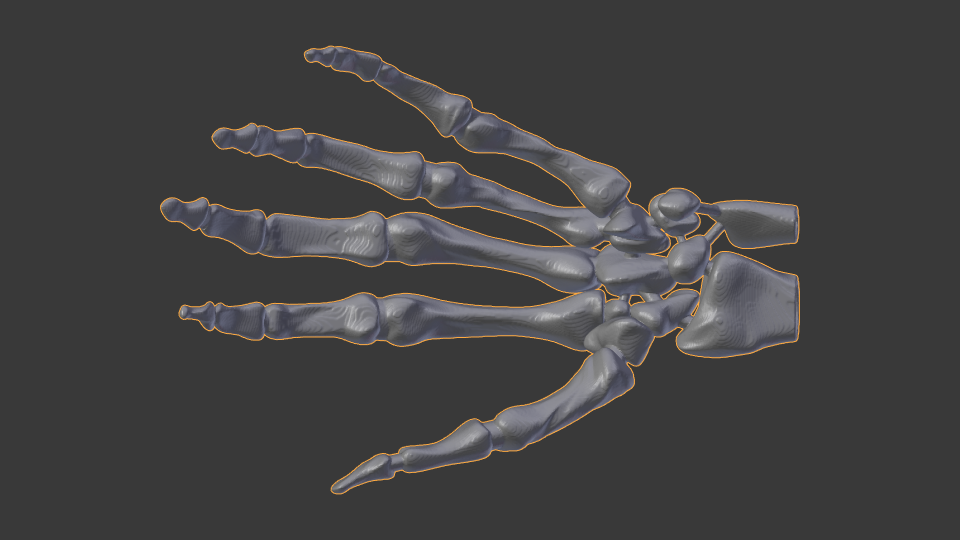
\includegraphics[trim={1.5in 0 1.5in 0},clip,height=2.5in]{images/hand}
	}
	\caption{
		(a),(b) Reconstructed Model with 757490 vertices and (c),(d) with 172974 vertices. (e) Rendered Image of a reconstructed surface with 327323 vertices.
	}
\end{figure*}
\begin{figure*}
	\centering
	\subfigure[\label{fig:bumpy0000}]{
		\includegraphics[trim={3.8in 0.8in 3.8in 0.8in},clip,height=2.3in]{images/bumpy/0000}
	}
	\subfigure[\label{fig:bumpy0001}]{
		\includegraphics[trim={3.8in 0.8in 3.8in 0.8in},clip,height=2.3in]{images/bumpy/0001}
	}
	\subfigure[\label{fig:bumpy0002}]{
		\includegraphics[trim={3.8in 0.8in 3.8in 0.8in},clip,height=2.3in]{images/bumpy/0002}
	}
	\subfigure[\label{fig:bumpy0003}]{
		\includegraphics[trim={3.8in 0.8in 3.8in 0.8in},clip,height=2.3in]{images/bumpy/0003}
	}
	\subfigure[\label{fig:bumpy0004}]{
		\includegraphics[trim={3.8in 0.8in 3.8in 0.8in},clip,height=2.3in]{images/bumpy/0004}
	}
	\subfigure[\label{fig:bumpy0005}]{
		\includegraphics[trim={3.8in 0.8in 3.8in 0.8in},clip,height=2.3in]{images/bumpy/0005}
	}
	\subfigure[\label{fig:bumpy0006}]{
		\includegraphics[trim={3.8in 0.8in 3.8in 0.8in},clip,height=2.3in]{images/bumpy/0006}
	}
	\subfigure[\label{fig:bumpy0007}]{
		\includegraphics[trim={3.8in 0.8in 3.8in 0.8in},clip,height=2.3in]{images/bumpy/0007}
	}
%	\subfigure[\label{fig:bumpy0008}]{
%		\includegraphics[trim={3.8in 0.8in 3.8in 0.8in},clip,height=2in]{images/bumpy/0008}
%	}
	\subfigure[\label{fig:bumpy0009}]{
		\includegraphics[trim={3.8in 0.8in 3.8in 0.8in},clip,height=2.3in]{images/bumpy/0009}
	}
	\caption{
		Surface during Iteration of bumpy Sphere.
	}
\end{figure*}
\begin{figure*}
	\centering
	\subfigure[\label{fig:plane0000}]{
		\includegraphics[trim={1in 0.5in 1in 0.5in},clip,height=1.5in]{images/plane/0000}
	}
	\subfigure[\label{fig:plane0001}]{
		\includegraphics[trim={1in 0.5in 1in 0.5in},clip,height=1.5in]{images/plane/0001}
	}
	\subfigure[\label{fig:plane0002}]{
		\includegraphics[trim={1in 0.5in 1in 0.5in},clip,height=1.5in]{images/plane/0002}
	}
	\subfigure[\label{fig:plane0003}]{
		\includegraphics[trim={1in 0.5in 1in 0.5in},clip,height=1.5in]{images/plane/0003}
	}
	\subfigure[\label{fig:plane0004}]{
		\includegraphics[trim={1in 0.5in 1in 0.5in},clip,height=1.5in]{images/plane/0004}
	}
	\subfigure[\label{fig:plane0005}]{
		\includegraphics[trim={1in 0.5in 1in 0.5in},clip,height=1.5in]{images/plane/0005}
	}
	\subfigure[\label{fig:plane0006}]{
		\includegraphics[trim={1in 0.5in 1in 0.5in},clip,height=1.5in]{images/plane/0006}
	}
	\subfigure[\label{fig:plane0007}]{
		\includegraphics[trim={1in 0.5in 1in 0.5in},clip,height=1.5in]{images/plane/0007}
	}
	%	\subfigure[\label{fig:plane0008}]{
	%		\includegraphics[trim={1in 0.5in 1in 0.5in},clip,height=2in]{images/plane/0008}
	%	}
	\subfigure[\label{fig:plane0009}]{
		\includegraphics[trim={1in 0.5in 1in 0.5in},clip,height=1.5in]{images/plane/0009}
	}
	\caption{
		Surface during Iteration of Plane.
	}
\end{figure*}

%\bibliographystyle{elsarticle-num}
%\bibliography{references}



\end{document}